%AGAIN: put STG, COG, or ADG here depending on the call
\documentclass[B2,COG]{ercgrant}
% put here the year of the call

\renewcommand{\callyear}{2023}
\setmainfont{Arial}
\bibliography{bibliography.bib}
\bibliography{bibliography_pawel.bib}

% \author{Fabian Sinz}
% \acro{Visual System in Action}
% \title{Data-driven embodied digital twins of mouse visual cortex.}
% \institution{Georg August Universität Göttingen}

\newcommand{\oonetitle}{An video-driven digital twin of mouse visual cortex during free behavior}
\newcommand{\otwotitle}{Find tuning changes and characterize uncertainty in latent dimensions}
\newcommand{\othreetitle}{Identify causal links between neural representations and behavior}
\author{Fabian Sinz}
\acro{Visual System in Action}
% \title{Putting data-driven digital twins of mouse visual cortex into action.}
% \title{Towards a meta-verse for the mouse visual system}
% \title{Building a data driven model how behavior changes neuronal processing in mouse visual cortex in freely behaving mice}
\title{A data-driven characterization of free behavior's impact on mouse visual processing}
\institution{Georg August Universität Göttingen Stiftung Öffentlichen Rechts}

% \renewcommand{\callyear}{2050}

% \author{\textcolor{red}{Dr. Jane/John Doe}}
% \acro{\textcolor{red}{ACRONYM}}
% \title{\textcolor{red}{PROJECT TITLE}}
% \institution{\textcolor{red}{Example Institute}}

% ====== BODY OF THE DOCUMENT ======
\begin{document}

\maketitle

%%%%%%%%%%%%% PART B 2 %%%%%%%%%%%%%%%%%%%


\chapter{The Scientific Proposal}


%%%%%%%%%%%%% STATE-OF-THE-ART %%%%%%%%%%%%%%%%%%%
\section{State-of-the-art and objectives}\label{sec:stateofart}
\subsection{Building a bridge between visual representations and behavior}
The goal of the visual system is to extract actionable information about our environment from the complex and ambiguous light patterns that inform our brain about the world beyond our eyes.
However, vision is not a one-way street: The activity of each neuron in the visual system is not only determined by visual input, but also changes with the internal state or motor behavior of the animal~\parencite{Niell2010-bs, Musall2019-kd, Erisken2014-un, Franke2022-do}, even when the animal's head is fixed to the experimental device~\parencite{Stringer2019-lt, Musall2019-kd} -- like in vast majority of neuroscience experiments.
Currently there is a trend towards studying vision by recording from freely moving animals and naturalistic stimuli~\parencite{Parker2022-ac,Holmgren2021-jv}. 
However, analyzing these data poses new computational challenges~\parencite{Busse2017-rt}. 
Thus, how and when motor behavior influences visual representations in freely viewing and behaving animals is currently an open question. 
%
The goal of this proposal is to investigate the hypothesis that \textbf{neurons in mouse visual cortex adapt their stimulus preference to the current motor behavior to in order to decrease uncertainty about momentarily relevant aspects of the world.} 

Studying vision under free behavior~\parencite{Parker2022-ac}, poses new challenges. 
Experimental conditions and behavior cannot easily be controlled or repeated like in classical trial structures~\parencite{Huk2018-ez}, and complex natural visual input is not easily parametrized. 
In addition, studying whether a neuronal mechanism is \textit{necessary} for  behavior usually involves a prediction how shutting down the mechanism affects the performance of an animal in elaborate behavioral tasks the animals need to be trained for.
During unconstrained behavior, the animal might simply adapt its behavior to compensate for the experimental intervention, changing both the performance and motor behavior in non-trivial ways.  
Making a prediction about these changes is challenging.
% While this makes investigating how \textit{behavior affects neuronal representations} already challenging enough, studying the \textit{computational necessity} of visual represenations for behavior is even more challenging.
% This is because it involves a fundamentally causal question: Given that the animal wants to achieve a particular behavioral goal, how would its behavioral strategy change if particular mechanisms of visual representation were changed or turned off?
To tackle these challenges, I propose to \textbf{build a computational framework based on data-driven deep neural network models of the visual system, detailed motor behavior captured by posture graphs of freely behaving mice, digital replicas of real environments and reinforcement learning}.
% \begin{figure*}[b]
% 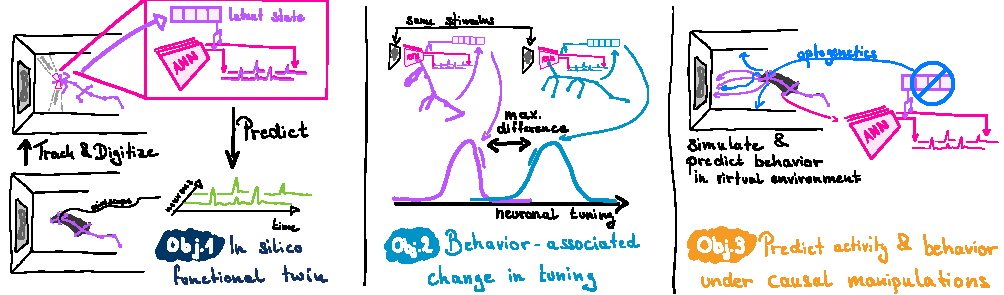
\includegraphics[width=\textwidth]{figures/overview5.pdf}
% \end{figure*}
My team and I will build a model for visual cortex under free behavior (\obj{1}), use it to disentangle the contribution of visual input, behavior, and internal state to neuronal activity, and study how motor behavior, internal state and task context affects neuronal stimulus selectivity (\obj{2}). To study the behavioral relevance of these selectivity-changes, I will use reinforcement learning to predict how shutting them down affects behavioral strategies and performance of mice in an open field object recognition task  (\obj{3}, Fig.~\ref{fig:openfield}).


\subsection{Visual cortex in the context of internal state, and behavior}

Sensory systems provide the informational basis of behavior: Their incomplete and noisy image of the environment is our only way to make decisions and pick the next action based on environmental information. 
At the same time, the brain can choose what to measure: Our actions influence the input to our senses and sensory processing itself adapts to the current behavioral needs. 

% 

The fact that sensory processing changes with motor activity and internal state was first demonstrated by elegant studies on invertebrates many decades ago  \parencite{Rowell1971-zj, Wiersma1968-xt}.
Since then, modulation of sensory responses as a function of behavioral and internal state, such as attention, has been described in many animals \parencite[\eg][]{Maimon2010-sa, Niell2010-bs,Bezdudnaya2006-ge, Treue1996-lp, Musall2019-kd}.
In many cases, state-dependent modulation affects neural responsiveness, called \textit{gain}~\parencite{Eggermann2014-xp, Niell2010-bs, McAdams1999-cs,Schroder2020-jl, Dadarlat2017-jw, Mineault2016-fk}.
In other cases, however, the stimulus selectivity of single neurons are also affected by this modulation. 
In the visual system, this has been reported, for instance, for temporal tuning in Drosophila \parencite{Chiappe2010-bm}, rabbits \parencite{Bezdudnaya2006-ge}, and mice \parencite{Andermann2011-vw}, as well as for direction selectivity in primates \parencite{Treue1996-lp}.
Using more ethological UV-color stimuli and data-driven deep network models, we recently showed that arousal -- correlated with a dilated pupil and running -- can change stimulus selectivity of neurons in mouse visual cortex at the timescale of seconds~\parencite{Franke2022-do}. 
\textcite{Stringer2019-lt} recently showed that spontaneous neuronal population activity is modulated by multi-dimensional latent fluctuations, related to detailed motor activity of the animal~\parencite{Syeda2022-bk}.
Using an auditory and visual decision making task, \textcite{Musall2019-kd} found that task-irrelevant motor behavior becomes increasingly locked to the task and strongly modulates neuronal activity across the.
These studies demonstrate that, even in head-fixed animals, where behavioral options are limited and other cues, such as self-motion and vestibular signals, are missing, activity in visual cortex and other sensory areas is heavily influenced by motor activity.
This hints at an even richer repertoire of how behavior can affect visual processing in freely moving animals in complex environments~\parencite{Busse2017-rt,Huk2018-ez, Datta2019-qj}.
However, \textit{whether} and \textit{how} neurons in the visual system change their stimulus selectivity with motor behavior during free behavior is an open question. 
% Using functional twins based on deep neuronal networks, we recently showed that arousal -- correlated with a dilated pupil and running -- can differentially change the stimulus selectivity of subpopulations of neurons in mouse primary visual cortex at the timescale of seconds~\parencite{Franke2022-do}, adding more detail to previous work which reported an influence on the firing rate only~\parencite{Stringer2019-lt}\hl{leave?}.
% However, almost all previous work on the influence of behavior on visual representations have been performed in restrained animals, 
% Given that changes in tuning is a widespread phenomenon, I hypothesize that  that there are more ways how neuronal representations in mouse visual cortex changes with behavior. 
% A systematic characterization of the correspondence between behavioral context and visual representations during free behavior is currently missing. 

Why do visual representations change with behavior? 
% From the perspective of encoding and decoding visual signals, it might seem puzzling to change the encoder because the decoder would need to change, too. 
% Given that changes in visual representation are temporary suggests that sensory certainty is a limited resource that has to be spent wisely depending on the behavioral context.
A likely answer can come from behavior itself:
% However, including behavior can offer a possible explanation: 
When actions need to be chosen on the basis of uncertain sensory information about the world, decreasing uncertainty about momentarily relevant aspects becomes important~\parencite{Chebolu2022-tb}. 
If decreasing uncertainty comes at a cost -- energy or opportunity --, it makes sense to selectively bias visual processing depending on behavioral context, such as boosting higher temporal frequencies during walking, running, and flying.
% , \textit{e.g.} focusing on  higher temporal frequencies during walking, running, and flying periods.
Many known non-visual modulations of neural activity can be understood in that way: 
For instance, when attention increases neural activity in certain neurons, it also selectively increases their signal-to-noise ratio. 
In fact, previous studies reported that modulation of sensory responses resulted in better behavioral performance \parencite{Spitzer1988-kq, Bennett2013-rk, Dadarlat2017-jw, De_Gee2022-ir}.
% In these cases, the visual system might bias processing towards visual features relevant for current behavioral goals
The fact that most changes in representation are temporary suggests that certainty is a limited resource that has to be spent wisely depending on the behavioral context.
However, this means that the change of tuning becomes dependent on behavior.
Thus understanding \textit{which} neurons change their tuning with behavior, \textit{how} they change it, and  \textit{when},  will yield insights into the role these neurons play under natural conditions. \hl{we need to make sense of the tuning change in high dimensions}

To understand how visual processing adapts to natural motor behavior, we need to study neuronal representations under conditions that engage the full computational apparatus of the visual system~\parencite{Huk2018-ez, Datta2019-qj}. 
This means we have study how the response of neurons in the visual systems changes in freely behaving (unrestrained) animals using the complex natural visual input~\parencite[\eg][]{Parker2022-ac}.
% While the vast majority of visual neuroscience still uses head-fixed animals, minimalistic artificial stimuli (such as Gabor patches), and simple tasks (such as 2AFC) 
% there is a trend towards large scale recordings in freely behaving 
 % animals~\parencite[\eg][]{Parker2022-ac}.
However, this poses new challenges for the analysis of these experiments:
% However, this data poses new challenges:
% \begin{itemize}
    % \item 
    
\textit{Disentangling contributing factors of neuronal activity:}
At any point in time the neuronal activity in the visual system is the result of many factors, such as visual input, motor behavior, or internal state. 
To understand how they shape visual processing, we need to disentangle their contributions to the activity of neurons during free behavior. 
This includes reconstructing what the animal saw at every moment of the experiment, and developing models that can capture common fluctuations in neuronal population activity due to motor behavior or internal state in the neuronal population activity.

\textit{Gaining insights from non-repeatable trials} 
To characterize how neuronal representations changes with behavior in a classical experimental trial structure, one would need to present the same stimuli in different behavioral contexts. 
However, behavior and visual input in natural conditions cannot easily be controlled or repeated, and natural stimuli are not easily parametrized.
% \end{itemize}

\hl{we need models that can merge it, so far they were linear}

\subsection{Functional twins: Data-driven models of visual cortex and behavior}
One way to address both challenges is to compile many unique behavioral and physiological observations (possibly from multiple experiments) into a single computational model -- a data-driven \textbf{functional twin} -- that allows us to characterize neuronal representations \textit{in silico} and make specific predictions that are testable \textit{in vivo}. 
Functional twins are descriptive models that faithfully predict measurable observations for a real system, such as neural activity or behavior, and extrapolate over a large range of conditions, \textit{e.g.} arbitrary videos or behaviors. 
Thus, a functional twin mimics the system \textit{functionally}, without necessarily resembling it \textit{structurally}, like a biophysical circuit simulation.  

Descriptive models of neuronal function have a long history in systems neuroscience.
Prominent examples include linear nonlinear models of retinal ganglion cells~\parencite{Paninski2004-ax,Pillow2008-me}, quadratic energy models of complex cells~\parencite{Adelson1985-re}, divisive normalization models to account for complex contextual modulations~\parencite{Heeger1992-xx}, or subunit/LN-LN models~\parencite{Rust2005-ro,Touryan2005-pi,Vintch2015-gc}.
While these models do not have biophysically meaningful components, they still have a low number of interpretable parameters, like a linear filter. 
However, while these models yielded good predictions for earlier stages of the visual system or particular stimulus sets (like Gabors, gratings, or dot patterns), they are still quite constrained and often do not generalize well across different stimulus statistics~\parencite{Fournier2011-pl}, or cannot capture the complexities of neurons in higher visual areas.
To address that problem, one line of research  turned to more flexible multi-layer neural networks with more parameters~\parencite{Zipser1988-nh,Lehky1992-wf,Lau2002-gb,Prenger2004-qu}.
Like in many other areas of research, deep learning also led to tremendous progress in this area: task-optimized deep convolutional neural networks (CNNs) \parencite{Yamins2014-cg,Cadieu2014-gc,Cadena2017-rb} and CNN-based architectures learned end-to-end on physiological recordings set new standards in the prediction quality and extrapolation capability~\parencite{Antolik2016-va,Batty2016-do,McIntosh2016-tr,Klindt2017-sb,Kindel2017-xs,Cadena2017-rb,Burg2021-yg, Lurz2020-ua, Bashiri2021-or,Zhang2018-cs,Cowley2020-cy,Ecker2018-gz, Sinz2018-sk, Walker2019-yw, Franke2022-do}. 


The use of models trained end-to-end on data from physiological experiments marks a paradigm shift from models with easily interpretable parameters to large models whose major goal is to functionally mimic the neuronal system as closely as possible.
To emphasize this intention, we call these models \textit{functional twins}. 
Functional twins allow us to outsource experimentally difficult operations on the animal to an \textit{in silico} experiment in the model, such as searching for optimal stimuli~\parencite{Walker2019-yw} or mapping out tuning functions and inveriances~\parencite{Baroni2022-fi}. 
However, it is important to note that the insights of such an \textit{in silico} experiment are usually easier to verify \textit{in vivo}. 
For instance, searching across the space of all image to find stimuli that strongly excite a given neuron is next to impossible in experiments because search space is so enormous.
However, using optimization, it is feasible in a model.
Once such an image has been found, it is easy to verify by simply showing it to the same animal again~\parencite{Walker2019-yw,Bashivan2019-ry}.
The unrealized potential of this approach to integrate complex experimental data, generate new predictions, and speed up our understanding of the brain is enormous. 
In fact, the authors of the \textit{neuroconnectionist research programme}~\parencite{Doerig2022-ex} advocated a ``large-scale research programme centered around ANNs as a computational language for expressing falsifiable theories about brain computation'' that generate ``new and otherwise unreachable insights into the workings of the brain''. 

% \begin{figure}[t]
% \floatbox[{\capbeside\thisfloatsetup{capbesideposition={right,top},capbesidewidth=0.3\textwidth}}]{figure}[\FBwidth]
% {\caption{Basic architecture of the existing video based predictive model for head-fixed mice with, simple behavioral variables, and no latent state.}\label{fig:videomodel}}
% {\includegraphics[width=.68\textwidth]{figures/architecure_v15_raster.pdf}}
% \end{figure}




% \begin{figure*}[t]
%     \centering
%     \includegraphics[width=.9\textwidth]{figures/architecure_v15_raster.pdf}
%     \caption{Basic architecture of the existing video based predictive model for head-fixed mice with, simple behavioral variables, and no latent state.
%     % Neuronal activity from the visual system of mice watching natural videos is recorded using a wide-field two photon microscope. Video stimuli are fed to a deep recurrent neuronal network that provides a nonlinear feature representation shared among thousands of simple (linear-nonlinear) predictors, one for each neuron. Behavior, such as locomotion or pupil size in this example, can be part of the input to the model and adapt the feature representation. The input to the model can be adapted to the gaze of the animal predicted from the pupil position in an eye tracking video. As the mapping from pupil to gaze is learned simply by maximizing predictive performance, it does not require an additional calibration of an eye tracker.
%     }    
%     \label{fig:videomodel}
% \end{figure*}


\begin{wrapfigure}[19]{r}{.6\textwidth}
\includegraphics[width=\linewidth]{figures/architecure_v15_raster.pdf}
\caption{Basic architecture of the existing video based predictive model for head-fixed mice with, simple behavioral variables, and no latent state.}
\label{fig:videomodel}
\end{wrapfigure}
My group and I made key contributions to the development of data-driven models, trained end-to-end on neuronal responses and natural images or video~\parencite{Sinz2018-sk, Walker2019-yw, Lurz2020-ua, Bashiri2021-or, Lurz2022-up, Franke2022-do, Cobos2022-rr, Ecker2018-gz,Cadena2019-jw}. 
I developed the first deep model of primary visual cortex on natural video~\parencite{Sinz2018-sk}, which was also the first model to include simple forms of behavioral variables, such as running speed or pupil dilation, and the first to incorporate gaze prediction of the animal as part of an end-to-end trained model (see Fig.~\ref{fig:videomodel}). 
We were the first to combine fully image driven model with latent state models that capture common fluctuations caused by internal states~\parencite{Bashiri2021-or}.
In addition, we can infer boundaries between brain areas just from recordings of natural images, something that usually requires additional experiments~\parencite{Bashiri2021-or}.
We also demonstrated that these models learn characteristic feature representations for visual cortex that generalize well between neurons and animals~\parencite{Lurz2020-ua,Cobos2022-rr}.
Models based on our network architectures are currently state of the art in predicting mouse visual cortex\footnote{All winners of  \url{https://sensorium2022.net/} used our base network architecture}. 
Furthermore, we~\parencite{Walker2019-yw} developed the \textit{inception loops} paradigm that uses data-driven models of the visual system to synthesized new optimal stimuli for specific neurons that can readily be verified in follow-up experiments\footnote{Other groups from Harvard~\parencite{Ponce2019-yn} and MIT~\parencite{Bashivan2019-ry} concurrently published similar techniques for monkey visual cortex.}. 
Using this technique, we demonstrated that optimal stimuli for mouse primary visual cortex substantially deviated from previous text book models of visual tuning~\parencite{Hubel1959-zs}, and that selectivity of these neurons can change with arousal on the order of seconds~\parencite{Franke2022-do}.
Other labs are using our models to gather new insights about the visual system~\parencite{Hofling2022-wr} or model it under complex conditions~\parencite{Parker2022-ac}.


Functional twins allow neuroscience researchers to accurately model neuronal responses in passively viewing animals. 
However, the visual system is not a passive observer and many neuroscience experiments involve a task or behavior to understand causal effects of the visual representations onto the actions of an animal. 
Since behavioral experiments are often tedious and time consuming, and since it is hard to make predictions for natural unconstrained behavior, a modeling approach that integrates neuronal activity and flexible behavior would substantially accelerate neuroscience research. 
However, several keys steps for such a model are missing. 
To model the effect of behavior on visual processing, we need a model that can capture this effect. 
Since the number of simultaneously recordable neurons in freely behaving animals is still orders of magnitude lower than in head-fixed animals, training such a model from scratch on one experiment only likely would not realize the full predictive power of such a model. 
Thus, we need effective transfer learning schemes to pre-train a model on head-fixed data, where large scale data is available, and transfer it to freely behaving animals in a way that still allows us to capture how behavior influences visual processing. 
To model visual cortex under free viewing, we need to know the visual input to the mouse. 
This means we need to track experimentally its gaze, which is technically challenging, or we need to infer the gaze from video recordings of the animal and simultaneous recordings of neuronal activity. 
Furthermore, if we want to make predictions about how visual system about behavior, we need to provide the possibility for the model to behave differently than what we observed (to answer ``what if'' type of questions). 
This means we have to be able to predict the visual input from new viewpoints.
Existing approaches that mount a camera on a behaving mouse~\parencite{Parker2022-ac} do not allow for that. 
Other approaches that used a digitized environment, did not model neuronal activity~\parencite{Holmgren2021-jv}.
Finally, there is no previous work that combines a model of a real neuronal visual system with a model that selects actions of a mouse in free behavior. 
This is needed, however, to make predictions about how neuronal visual processing mechanisms affect behavior. 

\hl{models need video, latent state, and an environment that can ask what if questions?}

% modeling a visual system of a free running mouse that captures the effect of  during free behavior that captures the interaction requires a 
% \hl{What's the gap: Behavior and video. Latent states. Interaction between the two. }
% \hl{Simulation of different behavioral input}
% \hl{For behavior: What if the mouse did something else -> visual input changes  }

\subsection{Studying the effect of visual representations on behavior}
% virtual mouse, the paper by the guy from Freiburg, Deepmind paper, some Dayan work maybe?
The gold-standard in understanding the computational relevance of visual representations  is to quantify the effect of causal manipulations of the visual system on decisions and behavior. 
For instance, if changes in neuronal tuning serve to decrease uncertainty in relevant world dimensions, then disabling these changes should result in a higher variance or lower accuracy of the animal's performance in a task, or in some kind of compensatory behavior, such as longer decision times.
These kinds of questions involve many computational and experimental challenges. 
The first is to come up with a specific prediction for the behavioral effect of the causal manipulation: For instance, other neuronal circuits parallel or downstream of the manipulation might have complex effects on the decision of the behavior of an animal that can be hard to control. 
Second, to experimentally show the effect, animals need to be trained on a task which is time consuming and tedious. 
A computational framework that uses a functional twin to make specific behavioral predictions would tremendously speed up neuroscience research because it could be used to prescreen tasks and make more specific predictions, which are easier to test. 
Here, I propose to develop such an approach in \obj{3}. 

To answer causal questions about visual representations we need a behavioral goal (\eg~specified by a reward) and derive behavior from that. 
This is the domain of reinforcement learning.
There is a large literature that studies the neuronal basis of decisions and motor behavior of animals using reinforcement learning, imitation learning, or optimal control~\parencite{Schultz1997-xu,Todorov2004-yb, Morris2006-ub, Botvinick2009-nn, Yamaguchi2018-xp, Miyazaki2018-gy}\hl{more refs}.
For instance, \textcite{Kalweit2022-ev} recently demonstrated that accounting for the intrinsic reward inferred via inverse reinforcement learning and neuronal data can improve the predicted accuracy of a mouse's behavior by approximately 40\%.
However, all previous studies either assume that the state of the environment is known to the animal, use strongly simplified (low dimensional) sensory models, or study a very constrained environment with a severely limited action space. 

On the other hand, it has been demonstrated in the recent past that combining reinforcement learning algorithms with complex deep network based vision models is feasible. 
\textcite{Merel2020-hf} trained a virtual rat to perform tasks in a virtual environment and studied the effect of manipulating representations in the agent's visual system onto task behavior, and demonstrated that they could obtain meaningful results with ablating selected neurons in the circuit. 
\textcite{Deverett2019-gs} explored the effect of recurrence in an artificial neural network on behavior. 
They show that the ablation of recurrent connections removes the agents ability to internally measure time and instead the agent used rhythmic behavior to track time. 
Interestingly, measuring time by rhythmic motor behavior has been studied in animals behavior and known as stigmergy.
Finally, \textcite{Hilton2020-jz} showed that altering the image feature extractor model of a reinforcement learning agent results in predictable changes of behavior.
While all of these machine learning studies demonstrate that the effect of altering the ``visual system'' of a virtual agent on behavior can be systematically studied, none of these studies use neuronal data, realistic models of a visual system, or real behavior of animals. 
A computational framework that integrates large scale neuronal activity in the visual system and behavior in a realistic environment or task, is thus timely, but currently non-existent. 
% The mouse is an almost perfect model system for this.
% The absence of a fovea and the relatively low resolution of the visual system makes it easier to model its visual system, and the genetic toolbox available offer many opportunities to test the effect of causal manipulations onto behavior \textit{in vivo}.
\hl{we need a model that can ask what if questions for behavior}
\subsection{Objectives}
The proposed project is centered around three central questions, addressed in three objective:
\obj{1} What are the contributions of visual stimulus, motor behavior, and internal state to neuronal activity in freely moving mice?
\obj{2} How does neuronal tuning in visual cortex change with motor behavior or behavioral context?
\obj{3} Are changes in neuronal tuning necessary to explain goal-driven behavior and task performance?
% To answer these questions, I propose to map out the correspondence between changes in neuronal tuning and behavioral context during spontaneous and goal-driven behavior using data-driven functional twins of mouse visual cortex merged with detailed behavior described by posture graphs in digitized environments.
% % such that changes of visual computations with behavior and internal state are preserved. 
% Furthermore, I propose to develop a computational framework based on the model and reinforcement learning to make causal predictions about the behavioral relevance of these mechanisms. 
This results in the following goals:

% \begin{itemize}[leftmargin=2em,topsep=0pt,itemsep=0.62ex,partopsep=0ex,parsep=0.5ex,rightmargin=1ex]
\obj{1} \textbf{\oonetitle} to \textbf{disambiguate the contributions of stimulus, behavior, and internal state} to neuronal responses in miniscope recordings of freely moving animals. This model will form the backbone for \obj{2} and \obj{3}.

\obj{2} \textbf{\otwotitle} and quantify which scene properties are represented more accurately as a result of a change in tuning. 
I expect a close correspondence between motifs of motor behavior and which scene aspects are more accurately represented. 

\obj{3} \textbf{\othreetitle} by letting the functional twin learn to solve an object recognition task with reinforcement learning and ablating tuning changes in the model. 
% We will validate the approach by modeling optogenetic interventions first and subsequently predict how behavior and task performance would change if the changes in tuning were turned off. 
I expect that disabling tuning changes in the model that are associated with behavioral motifs used in the task (as identified in \obj{2}) will lead to an increased uncertainty in task relevant variables and predict a change in behavior of the animal to compensate for that. 

\subsection{Significance}
% \subsubsection{Interdisciplinarity}

\textbf{Interdisciplinarity} 
Today, neuroscience can record more detail and volume  of  behavioral and physiological data than ever before, putting it in the area of big data. 
Fully unlocking the potential of these data, requires strong expertise in computational sciences, such as  machine learning, and in neuroscience. 
I am trained in bioinformatics (undergraduate), machine learning (since undergraduate), computational neuroscience (PhD), and neuroscience (postdocs).
% I was the coordinator for machine learning and computational neuroscience in a large consortium\footnote{Machine Intelligence from Cortical Networks: \url{https://ninai.org}} to understand the cortical algorithms of vision.
% This and multiple follow-up projects gives me access to >18M neuron-hours of responses to visual stimuli across the entire mouse visual cortex. 
% This project develops novel machine learning methods for fundamental research questions in neuroscience, and 
I will make sure that my students and postdocs will develop this expertise in both fields and maximally benefit from a interdisciplinary environment by enabling them to spend time in our experimental collaborators’ labs (Emmanouil Froudarakis at FORTH and Andreas Tolias at Baylor College of Medicine).
This will also enable them to test our computational predictions together with experimentalists.


\textbf{Beyond state of the art \& potential impact} 
The proposed project develops crucial computational technology to step away from the typical trial based structure of systems and behavioral neuroscience towards a ``natural neuroscience'' that focuses on studying a neural system under complex natural conditions that cannot easily controlled or repeated. 
If successful, it can change our view on visual cortex and how visual processing adapts to motor behavior. 
% Even in classical conditions every trial in a neuronal system depends on uncontrollable factors (e.g. internal state) and can thus not be exactly repeated~\parencite{Urai2022-fz}. 
% I advocate to embrace this complexity and build models that can compile many experiments in a single model, can disentangle different factors of neuronal processing, yet make specific and verifiable experimental predictions. 
It pushes multiple boundaries of model development in neuronal data science with many applications beyond this project. \circled[black][black][white]{1} Most current models for visual cortex focus on static images and are built for behaviorally restrained (head-fixed) animals. The video-based latent-state model from \obj{1} merges two major determinants of a neuronal system: stimulus driven neuronal activity and behavior.
It is straightforward to generalize to include other areas (such as motor or prefrontal areas), or stimulus modalities (such as olfaction or sound), or more detailed observations (such as whisking or biophysical body models). 
Importantly, it allows us to explore the interaction between vision and behavior in situations that were not part of the experiments.
\circled[black][black][white]{2} The use of reinforcement learning in combination with functional twins of visual cortex and causal manipulations (\obj{3}) is unprecedented, and offers an innovative way to bridge the gap between visual representations and behavior. The framework is readily generalizable to other tasks and questions and will be a powerful tool to investigate the link between sensory representations and behavior, and derive specific predictions about the change of behavior from causal manipulations of the neurons in the visual system.
\circled[black][black][white]{3} As the volume, detail, and complexity of neuroscientific and behavioral data is increasing, my approach is one important step towards a \textit{standard model of systems neuroscience}.
The framework will not replace experiments, but make it easier, faster and cheaper to generate specific predictions by first running experiments \textit{in silico} before verifying the predictions \textit{in vivo}.

\textbf{Ethics in AI and the use of animals}
The misuse of machine learning can negatively impact the lives of individuals with respect to privacy, discrimination or bias. 
My  project will develop computational tools for fundamental research in neuroscience. 
Thus, I do not anticipate any direct negative consequences regarding ethical concerns related to human rights and values.

Although, we study neuronal systems and use large scale neuronal data, my lab will not perform any animal experiments in this project, but obtains this data from our long time experimental collaborators (see \nameref{sub:data}). 
% The experiments for a large fraction of the data volume that we want to use for this project have already been recorded. 
They have or will be carried out in agreement with ethical regulations and protocols approved by \hl{Manolis FORTH} and Baylor College of Medicine Institutional Animal Care and Use Committee (IACUC).
%%%%%%%%%%%%% METHODOLOGY %%%%%%%%%%%%%%%%%%%
\section{Methodology}
\subsection{Data and data management}
\label{sub:data}
\hl{mention transgenic}
\begin{wrapfigure}[8]{r}{.5\textwidth}
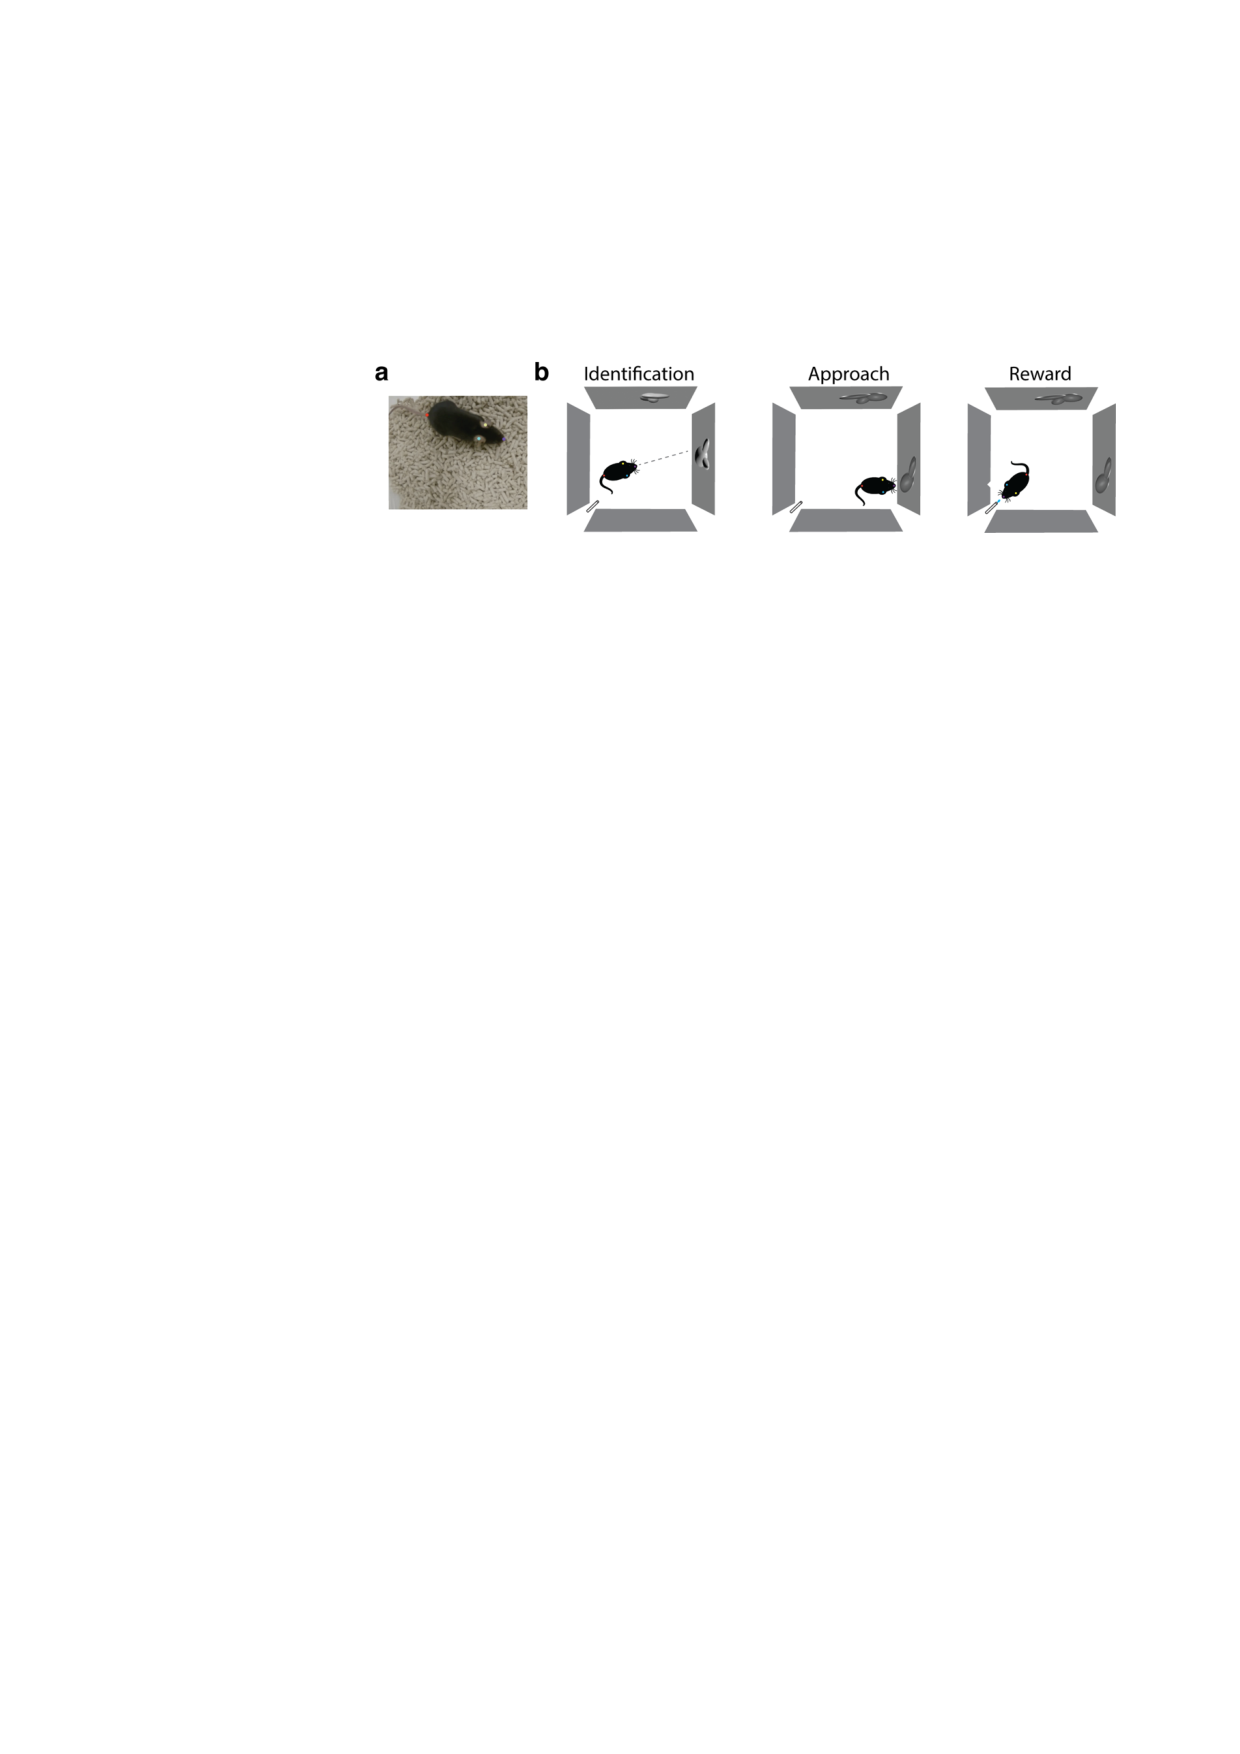
\includegraphics[width=\linewidth,trim=0 15 0 5, clip]{figures/openfield_ar.pdf}
\caption{Open field task: Animals have to identify the correct object and touch it to get water reward.}
\label{fig:openfield}
\end{wrapfigure}
This project at the frontier of machine learning and neuroscience would not be possible without actual neuroscientific and behavioral data. 
I have a long-standing collaboration with Dr. Tolias (Baylor College of Medicine, Houston, co-authors on >20  publications) and Dr. Froudarakis (FORTH, Crete, co-authors on >10 publications) who agreed to share physiological and behavioral data with me (see Letters of Support).
Our labs have a long and successful history of closely working together by exchanging data and machine learning models. 
Through Dr. Tolias, I have access to 2-photon recordings of more than 18M neuron hours of single cell resolution responses to visual stimuli across the entire visual cortex~\parencite{Sofroniew2016-xg}. A significant fraction of that is to natural video, recorded during the MICRONs project (\url{https://ninai.org}), which I was part of.
% In addition, he agreed to share behavioral tracking and neuropixel~\parencite{Steinmetz2021-jk} recordings from visual cortex in freely moving animals in an open arena that are currently being recorded in his lab.
Dr. Froudarakis will share data from miniscope~\parencite{Cai2016-rh}
recordings of freely behaving mice performing multiple open field object recognition tasks where animals can freely choose when to engage in the task (see \eg~Fig.~\ref{fig:openfield}). 
We will also use the episodes when the animal chooses not to perform the task to train our models. 
In addition, he will share physiological (and behavior) data from head-fixed or freely moving mice in which individual higher visual areas \hl{which} are optogenetically inhibited.
Dr. Froudarakis is currently recording these data as part of an ERC starting grant and other grants already awarded to him.\hl{prelim plot?} 
In addition, I have included a small budget for subcontracting supplementary experiments at the two labs (see letters of support).  
While the success of the project does not depend on these experiments, experimental verification of our predictions will make our results more impactful.
We will store, exchange and manage this data using \href{https://www.datajoint.org/}{DataJoint}~\parencite{Yatsenko2015-id}, an open source database system our labs developed. 
From ongoing collaborations the data management structure is established and ready to use.

\subsection{\colorbox{obj1}{\color{white}O1} Objective 1: \oonetitle}
\labelobj{1}

\textbf{Goal:} Build a functional digital twin of a mouse visual system to disentangle the contributions of visual input, behavior, and internal state to neuronal activity in visual cortex recorded during free behavior, and to simulate neuronal activity for novel behavioral trajectories.

\textbf{Overview and rationale:} Neuronal activity and tuning in visual cortex is not only determined by visual input, but can be profoundly affected by behavior and the internal state of an animal~\parencite{Niell2010-bs,Musall2019-kd,Stringer2019-lt, Franke2022-do}.
To disentangle the contributions from these different sources to neuronal activity in freely moving animals, I will move a deep video-based data-driven model of the mouse visual system through the digitized environment of the mouse according to its eye and body movement inferred from a behavioral video and pupil camera. 
While it is now possible to record hundreds of neurons during free behavior~\parencite{Parker2022-ac}, we are still not at the scale in terms of the number of neurons that can be reached with 2-photon. 
It might thus not be possible to train a video-based model only on the recordings from free behavior. 
To this end, I propose to use pre-train a video-based part on tens of thousands of excitatory neurons from multiple areas of the visual system recorded with 2-photon from head-fixed mice.
% and put it ``into the mouse's shoes'' by fitting it to recordings from a miniscope attached to a tracked stick-figure model of a freely behaving mouse in a  digitized version of its environment.
We will endow this model with an unobserved latent state that can capture variability due to non-visual signals~\parencite{Musall2019-kd, Bashiri2021-or} and possibly change tuning in visual neurons as a result.
When we attach the large scale model to the mouse in the digitized environment we will use the fewer neurons recorded during free behavior, fine tune it to the exact eye movements, and use the behavior to explain parts of the the non-visual neuronal variability captured by the latent state.

\begin{wrapfigure}[20]{r}{.35\textwidth}
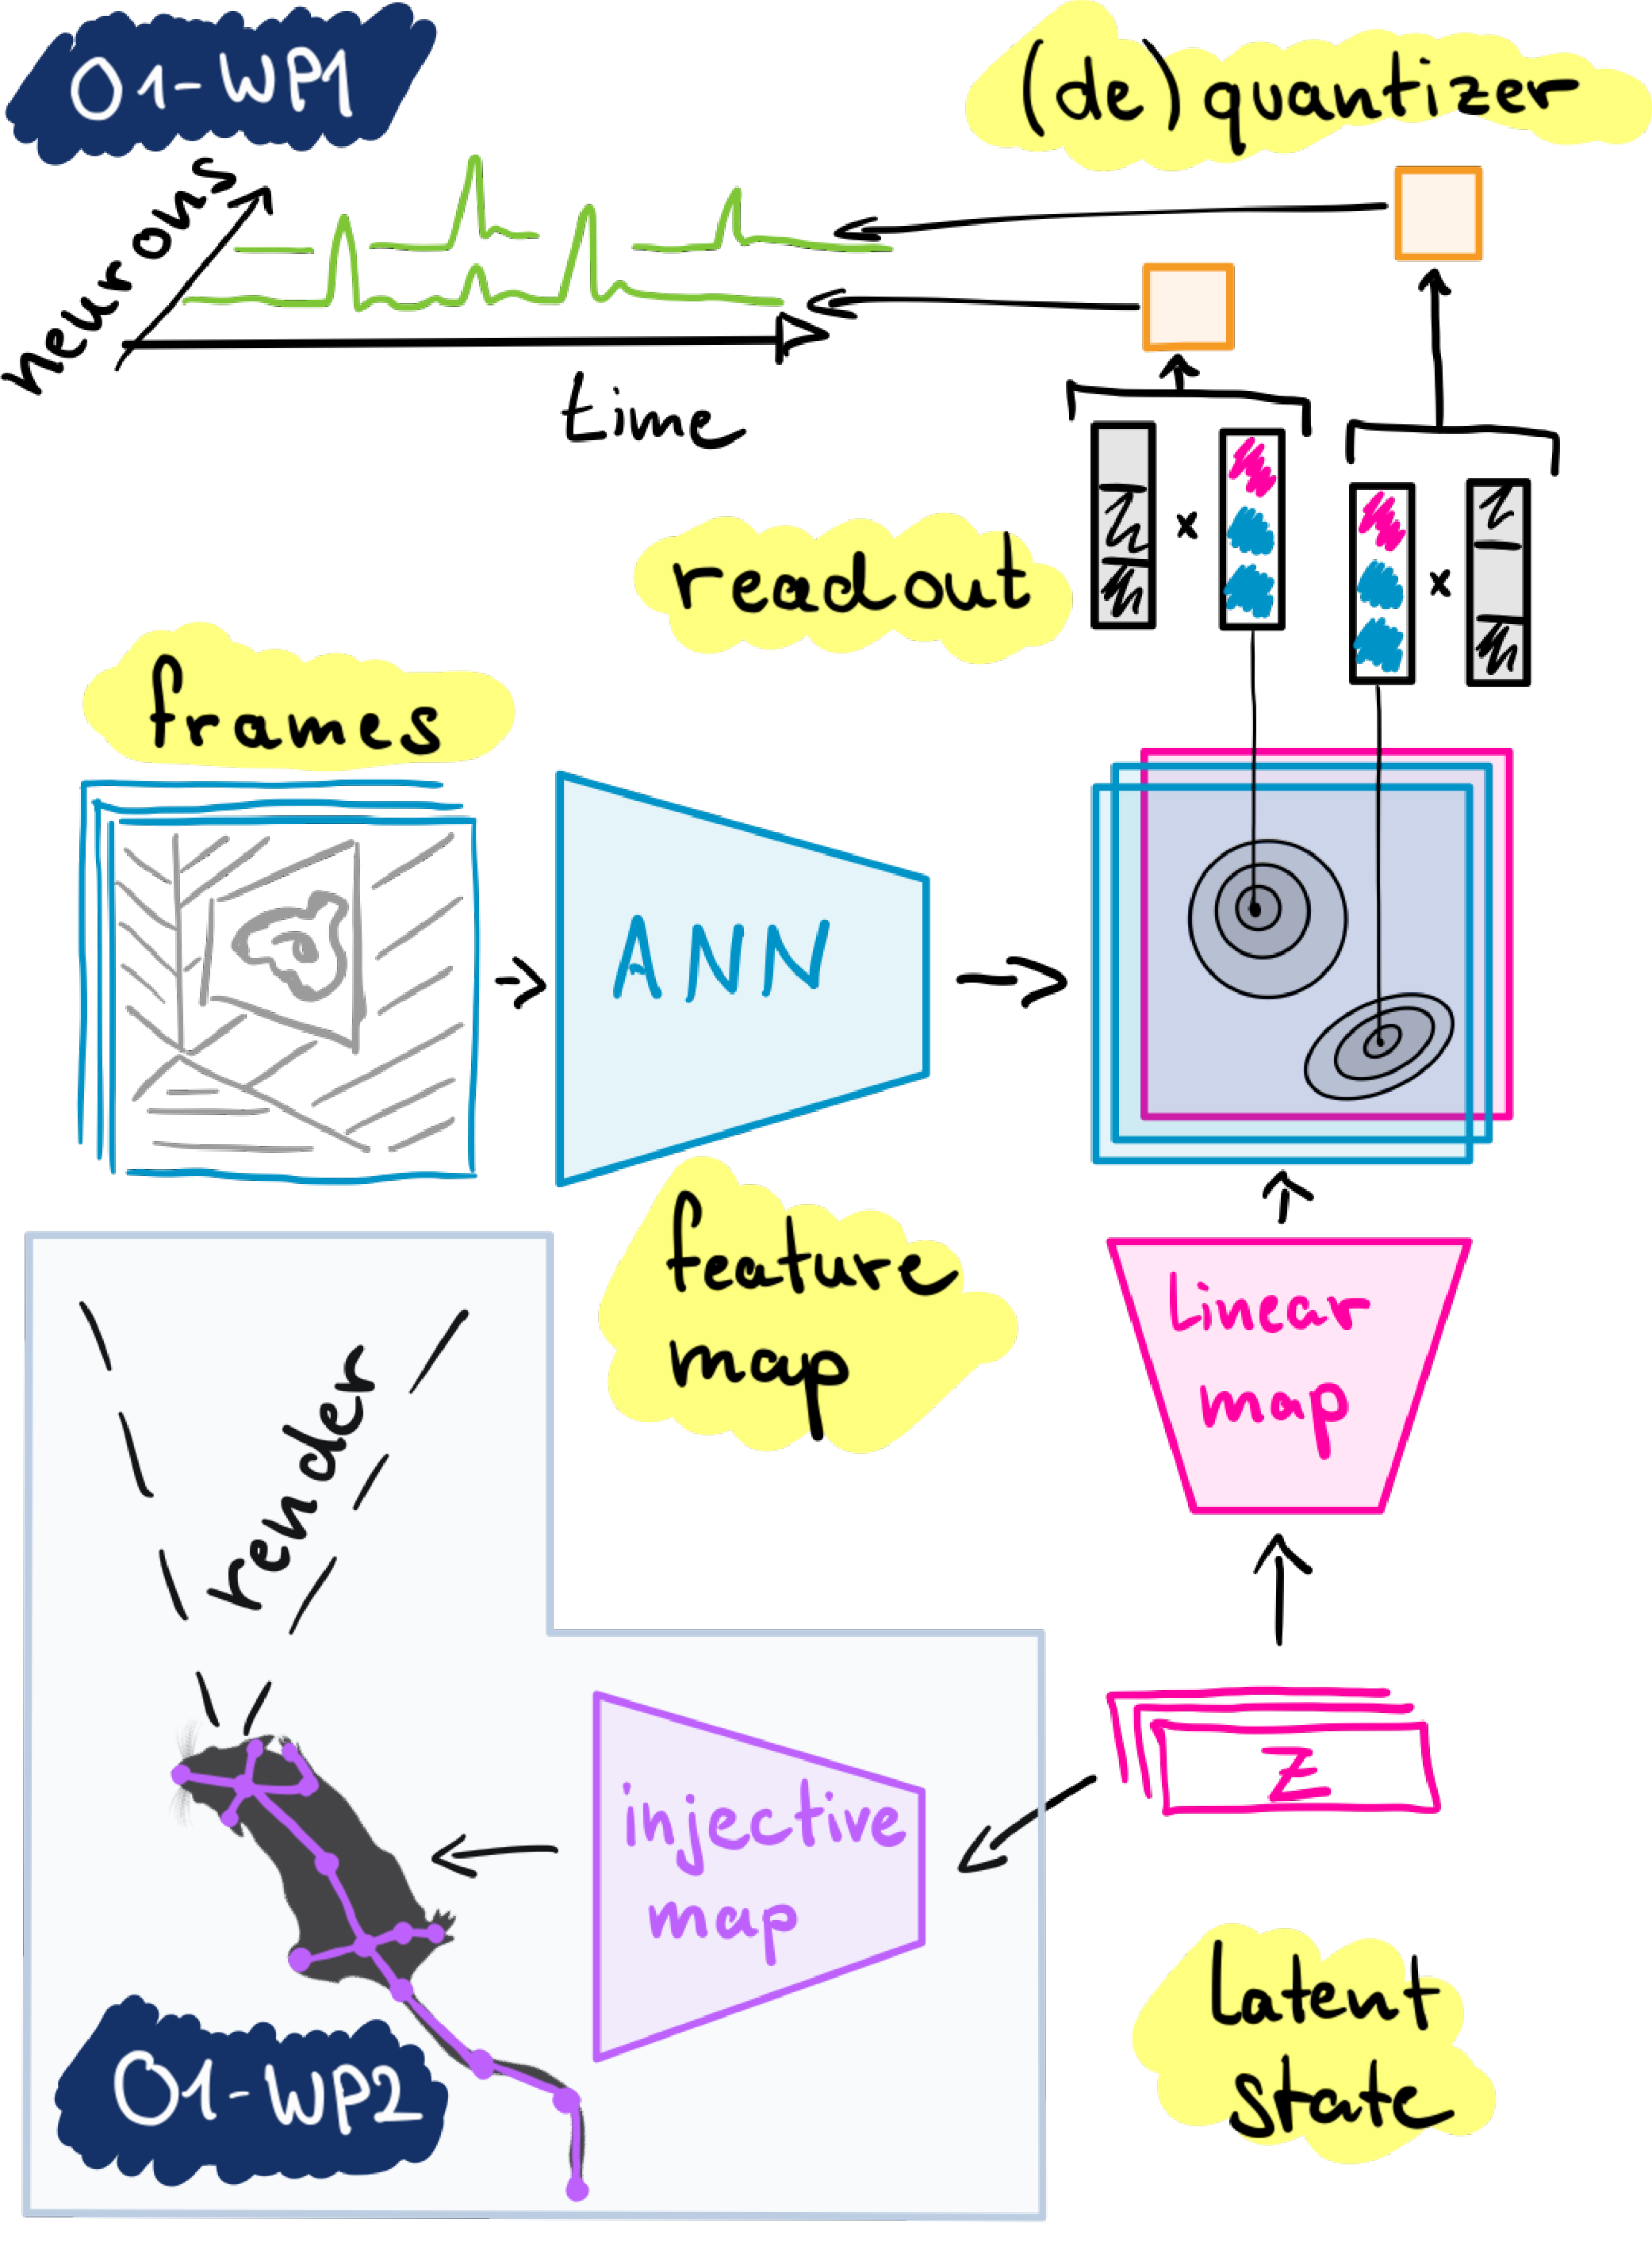
\includegraphics[width=\linewidth]{figures/model.pdf}
\caption{Schematic of the latent state video-driven model.\label{fig:model}}
\end{wrapfigure}
 

This approach offers several benefits:
% \begin{enumerate}[topsep=0pt,itemsep=0.62ex,partopsep=0ex,parsep=0.5ex]
    \circled[gray][gray][white]{1} We previously showed that models pre-trained on multiple datasets can be fit more efficiently to new neurons and stimuli using transfer learning~\parencite{Lurz2020-ua}. We thus expect pre-training to increase the predictive power. 
    \circled[gray][gray][white]{2} Since previous work has found the non-visual fluctuations to be relatively low dimensional compared to the number of neurons~\parencite{Stringer2019-lt}, we expect to identify the relevant dimensions in the head-fixed recordings first, and use the fewer neurons recorded with the miniscope to infer the actual state $\vec{z}$ in this lower dimensional space. We can then explain fluctuations in $\vec{z}$ via the actual behavior (by conditioning on it) and thus disentangle the contributions of visual input, behavioral state, and internal state to neuronal activity. 
    \circled[gray][gray][white]{3} The approach also allows us to put the visual system of the head-fixed mouse (with more neurons) onto the behaving mouse and use the latent state $\vec{z}$ inferred from the fewer neurons recorded during free behavior. 
    \circled[gray][gray][white]{4} The model in the digitized environment allows us to simulate neuronal activity for new behavioral trajectories that have not been observed in the data and even use the model as a virtual agent to simulate task driven behavior. An approach that directly mounts a camera on a mouse~\parencite{Parker2022-ac} cannot do that. 
% \end{enumerate}


The objective is split into three work packages. 
Building on my previous work~\parencite{Sinz2018-sk, Bashiri2021-or}, \objwp{1}{1} develops a video-driven latent state functional digital twin model. 
The technical innovation is to include a latent state into a dynamic model that can accurately capture low-dimensional population dynamics from non-visual sources, and can easily be adapted to new neurons and mice. 
\objwp{1}{2} digitizes the environment and infers the 3D trajectories of the animal's pose from video data.
\objwp{1}{3} builds the functional twin by attaching the pre-trained model to the mouse predicted eye positions, and fine-tuning it to neuronal activity and pupil positions recorded during free behavior.


% \textbf{Technical innovation:} This will be the first encoding model that predicts the activity of tens of thousands of neurons in visual cortex under free behavior and accounts for the modulation of neurons from brain state and behavior -- yielding an embodied functional digital twin that can be used to simulate new situations as close to real activity as currently possible.



\subsubsection{Work package 1.1: A video-driven latent state model of the visual system\hfill\objwp{1}{2}}
\labelobjwp{1}{1}
Like in my previous work, the video model will consist of a \textit{common feature map} that extracts nonlinear features from a given video using 3D convolutional and recurrent deep networks (Fig.~\ref{fig:model}).
To model common fluctuations in the neuronal population, we will add a Gaussian latent state $\vec{z}$ to this feature representation.
Correlations between neurons will be modeled by allowing the latent state to be correlated across space and time. 
In the image based model~\parencite{Bashiri2021-or}, we used a factor analysis model. 
To obtain an efficient dynamic model, we will either extend the factor analyzer to a finite window in time, or use a linear Gauss-Markov model. 
We will use a parameter efficient linear \textit{readout mechanisms} we developed~\parencite{Lurz2020-ua} to predict neuronal responses.
Since neural response have at least one discrete component (``0'' vs. other for two photon recordings), we will use variational dequantization~\parencite{Hoogeboom2021-zs} to make this discrete component continuous.
We will integrate over the latent state for fitting and train the model on the marginal likelihood of the transformed neural responses given the video.
This can be done efficiently because the latent state and the dequantized responses are linearly related.
Because of the variational dequantization (but not the latent state), we need to use variational inference to train the model on the marginal likelihood. 
We will train this model on large scale two-photon data from head-fixed mice watching natural, rendered, and noise movies.
This step will yield a video-driven latent-state foundation model for visual cortex that can be efficiently adapted to neurons recorded during free behavior.
% If necessary, we can also let the correlation structure depend on the visual input. 
% \hl{include what data the model is trained on, do we include behavioral state, or just compare to it.}

\subsubsection{Work package 1.2: Digitizing the environment and tracking behavior\hfill\objwp{1}{2}}
\labelobjwp{1}{2}



\textbf{Behavior via posture graph trajectories}
We will track the movement of the mouse in the cage from two cameras, and detect 2D keypoints of its posture graph using DeepLabCut~\parencite{Mathis2018-lk}. 
Subsequently, we will lift this 2D graph to a 3D posture graph using triangulation combined with a pose lifting model developed by us that can deal with temporarily occluded keypoints~\parencite{Pierzchlewicz2022-tq}. 
% For freely moving humans, this model achieves an accuracy of less than 5mm and can also deal with temporarily occluded keypoints. 
This step will yield a 3D trajectory of a stick-figure model of the mouse in its environment over time. 

\textbf{Digitize environment:} 
We will build a virtual model of the environment using LIDAR and baking images of the animal's cage as texture onto the scanned mesh~\parencite[similar as in][]{Holmgren2021-jv}.
% This is established technology can theoretically be done with an iPhone Pro 12, although we will purchase a more high-end solution.
Subsequently, we will use Blender and PyTorch3D to move our model in the environment according to the tracked movement of the mouse.
Since the cage and lab environment are standardized and static, we will not model the dynamics of the arena. 
However, we will include the monitor showing stimulus videos into the environment. 
This step will yield a virtual environment that we can use to recreate visual input from tracked or novel behavioral trajectories.


\subsubsection{Work package 1.3: Functional twin with behavior\hfill\objwp{1}{3}}
\labelobjwp{1}{3}

\textbf{Functional twin:} We will place the model learned from \objwp{1}{1} at the approximate eye locations of the mouse inferred from tracking the mouse and move it in the digitized environment according to the movement of the mouse. 
We will additionally account for the fact that mice do compensatory eye movements during locomotion\parencite[similar to rats][]{Wallace2013-lf} to get as close as possible to the true gaze position. 
We will then fine-tune the gaze position in each frame by optimizing the exact viewing direction of the rendering camera locations as a function of the pupil position of the mouse extracted from an additional camera mounted on the mouse's head.
We have already demonstrated before that end-to-end gaze inference is possible~\parencite{Sinz2018-sk,Walker2019-yw} and others have use this technique successfully in freely moving mice~\parencite{Parker2022-ac}.
% The fact that all neurons are affected by the gaze direction in the same way, makes it possible to identify the parameters from gaze 
For fine tuning the model to the pose trajectories, we will include them as an additional function of the latent state $\vec{z}$ to the model (Fig.~\ref{fig:model}). 
After fine tuning, this allows us to condition on the pose trajectories which makes them an input to the model. 
This yields a functional twin for neuronal activity during free behavior of a mouse.

\subsubsection{Expected outcome} 

An functional digital twin of the visual system of the mouse that allows us to disentangle the contributions of visual input, behavior, and internal state to neuron activity during free behavior. 
Importantly, it will allow us to discover behavior-associated changes in neuronal tuning functions by analyzing the influence of the posture graph on the predicted neuronal activity.
It will also allow us to predict neuronal activity to completely novel trajectories of the mouse in the environment.
We will quantify the prediction performance of the model by computing correlations of predicted neuronal activity with the actually recorded activity on episodes not used for training. 
As an additional quality control, we will predict the receptive fields of each neuron via gradients as in~\textcite{Sinz2018-sk}. 
If the model faithfully captures the response function of each neuron, we should see sharp receptive fields.
If not, the receptive fields will be smeared out~\parencite{Parker2022-ac}.

\subsubsection{Risk management} 
While \obj{1} will be a substantial step ahead, all single parts have been implemented on their own before by us~\parencite{Sinz2018-sk, Bashiri2021-or} or others~\parencite{Parker2022-ac,Holmgren2021-jv}. 
We thus expect to be able to successfully implement the model. 
If the latent state in head-fixed experiments should turn out to not be rich enough (\obj{1}), we will adapt it directly on data from multiple miniscope experiments. 
Using a forward facing and an eye camera in a mouse, \textcite{Parker2022-ac} already showed that they can account for eye movements and map receptive fields in behaving mice. Note, however, that they lack model for the interaction between behavior and vision, and they can only replay the path the mouse took (they could not do \obj{2} and \obj{3}).

Currently, our model only accounts for modulations due to motor behavior and any other non-visually driven activity is assigned to the internal state. 
However there might be other modalities that affect neuronal activity, such as proprioreception or whisking. 
Currently, our model will capture them under ``internal state''.
We will perform an additional analysis whether these factors have a major influence and include them in the model if necessary. 
We can estimate some proprioreception by inferring contact-to-ground from the behavior videos.
While it is unlikely that we can track single whiskers in the videos, we might be able to extract useful proxy features from the area around the head of the animal~\parencite{Syeda2022-bk}\hl{double check ref}.

%%%%%%%%%%%%%%%%%%%%%%%%%%%%%%%%%%%%%%%%%%%%%%%%%%%%%%%%%%%%%%%%%%%%%%%%%%%%%%
\subsection{\colorbox{obj2}{\textcolor{white}{O2}} Objective 2: \otwotitle}
\labelobj{2}


\textbf{Goals:} Find correspondence between change in neuronal tuning and stereotypical motor behavior or task context.
Describe scene properties that are encoded more accurately under the different tuning extremes. 

\textbf{Overview and rationale:} 
Behavior and state of arousal can modulate the response of neurons in mouse visual cortex~\parencite{Niell2010-bs, Stringer2019-lt, Musall2019-kd}.
We have recently demonstrated that tuning of neurons to color in mouse V1 can change with the behavioral state of the animal~\parencite{Franke2022-do}.
Previous studies reported that modulation of sensory responses resulted in better behavioral performance \parencite{Spitzer1988-kq, Bennett2013-rk, Dadarlat2017-jw, De_Gee2022-ir}.
I thus hypothesize that there are more ways how visual tuning adapts to behavior, and that this serves to decrease the uncertainty about stimulus dimensions that are relevant for the particular behavior. 
However, how motor behavior affects tuning in freely moving animals is an open question.
In addition, describing scene properties that are better encoded as a result of the tuning-change will also yield important clues about the behavioral goals of the mouse. 
In this objective I will use the trained functional twin model from~\obj{1} to discover correspondences between neuronal tuning in visual cortex and motor behavior in a data-driven way. 
We will use data from animals performing an open field object recognition task. 
To assess whether tuning changes could be induced by task context instead of motor behavior, we will additionally condition on task variables or only analyze episodes where the animal did not engage in the task. 
To quantify how the discovered changes in tuning affect the encoding of a scene, we will reconstruct geometric and semantic properties of the digitized scene from the activity in the model and quantify which scene properties are encoded more accurately. 


\subsubsection{Workpackage 2.1: Find behavior-associated change in visual tuning.\hfill \objwp{2}{1}}
\labelobjwp{2}{1}
%
\begin{wrapfigure}[20]{r}{.35\textwidth}
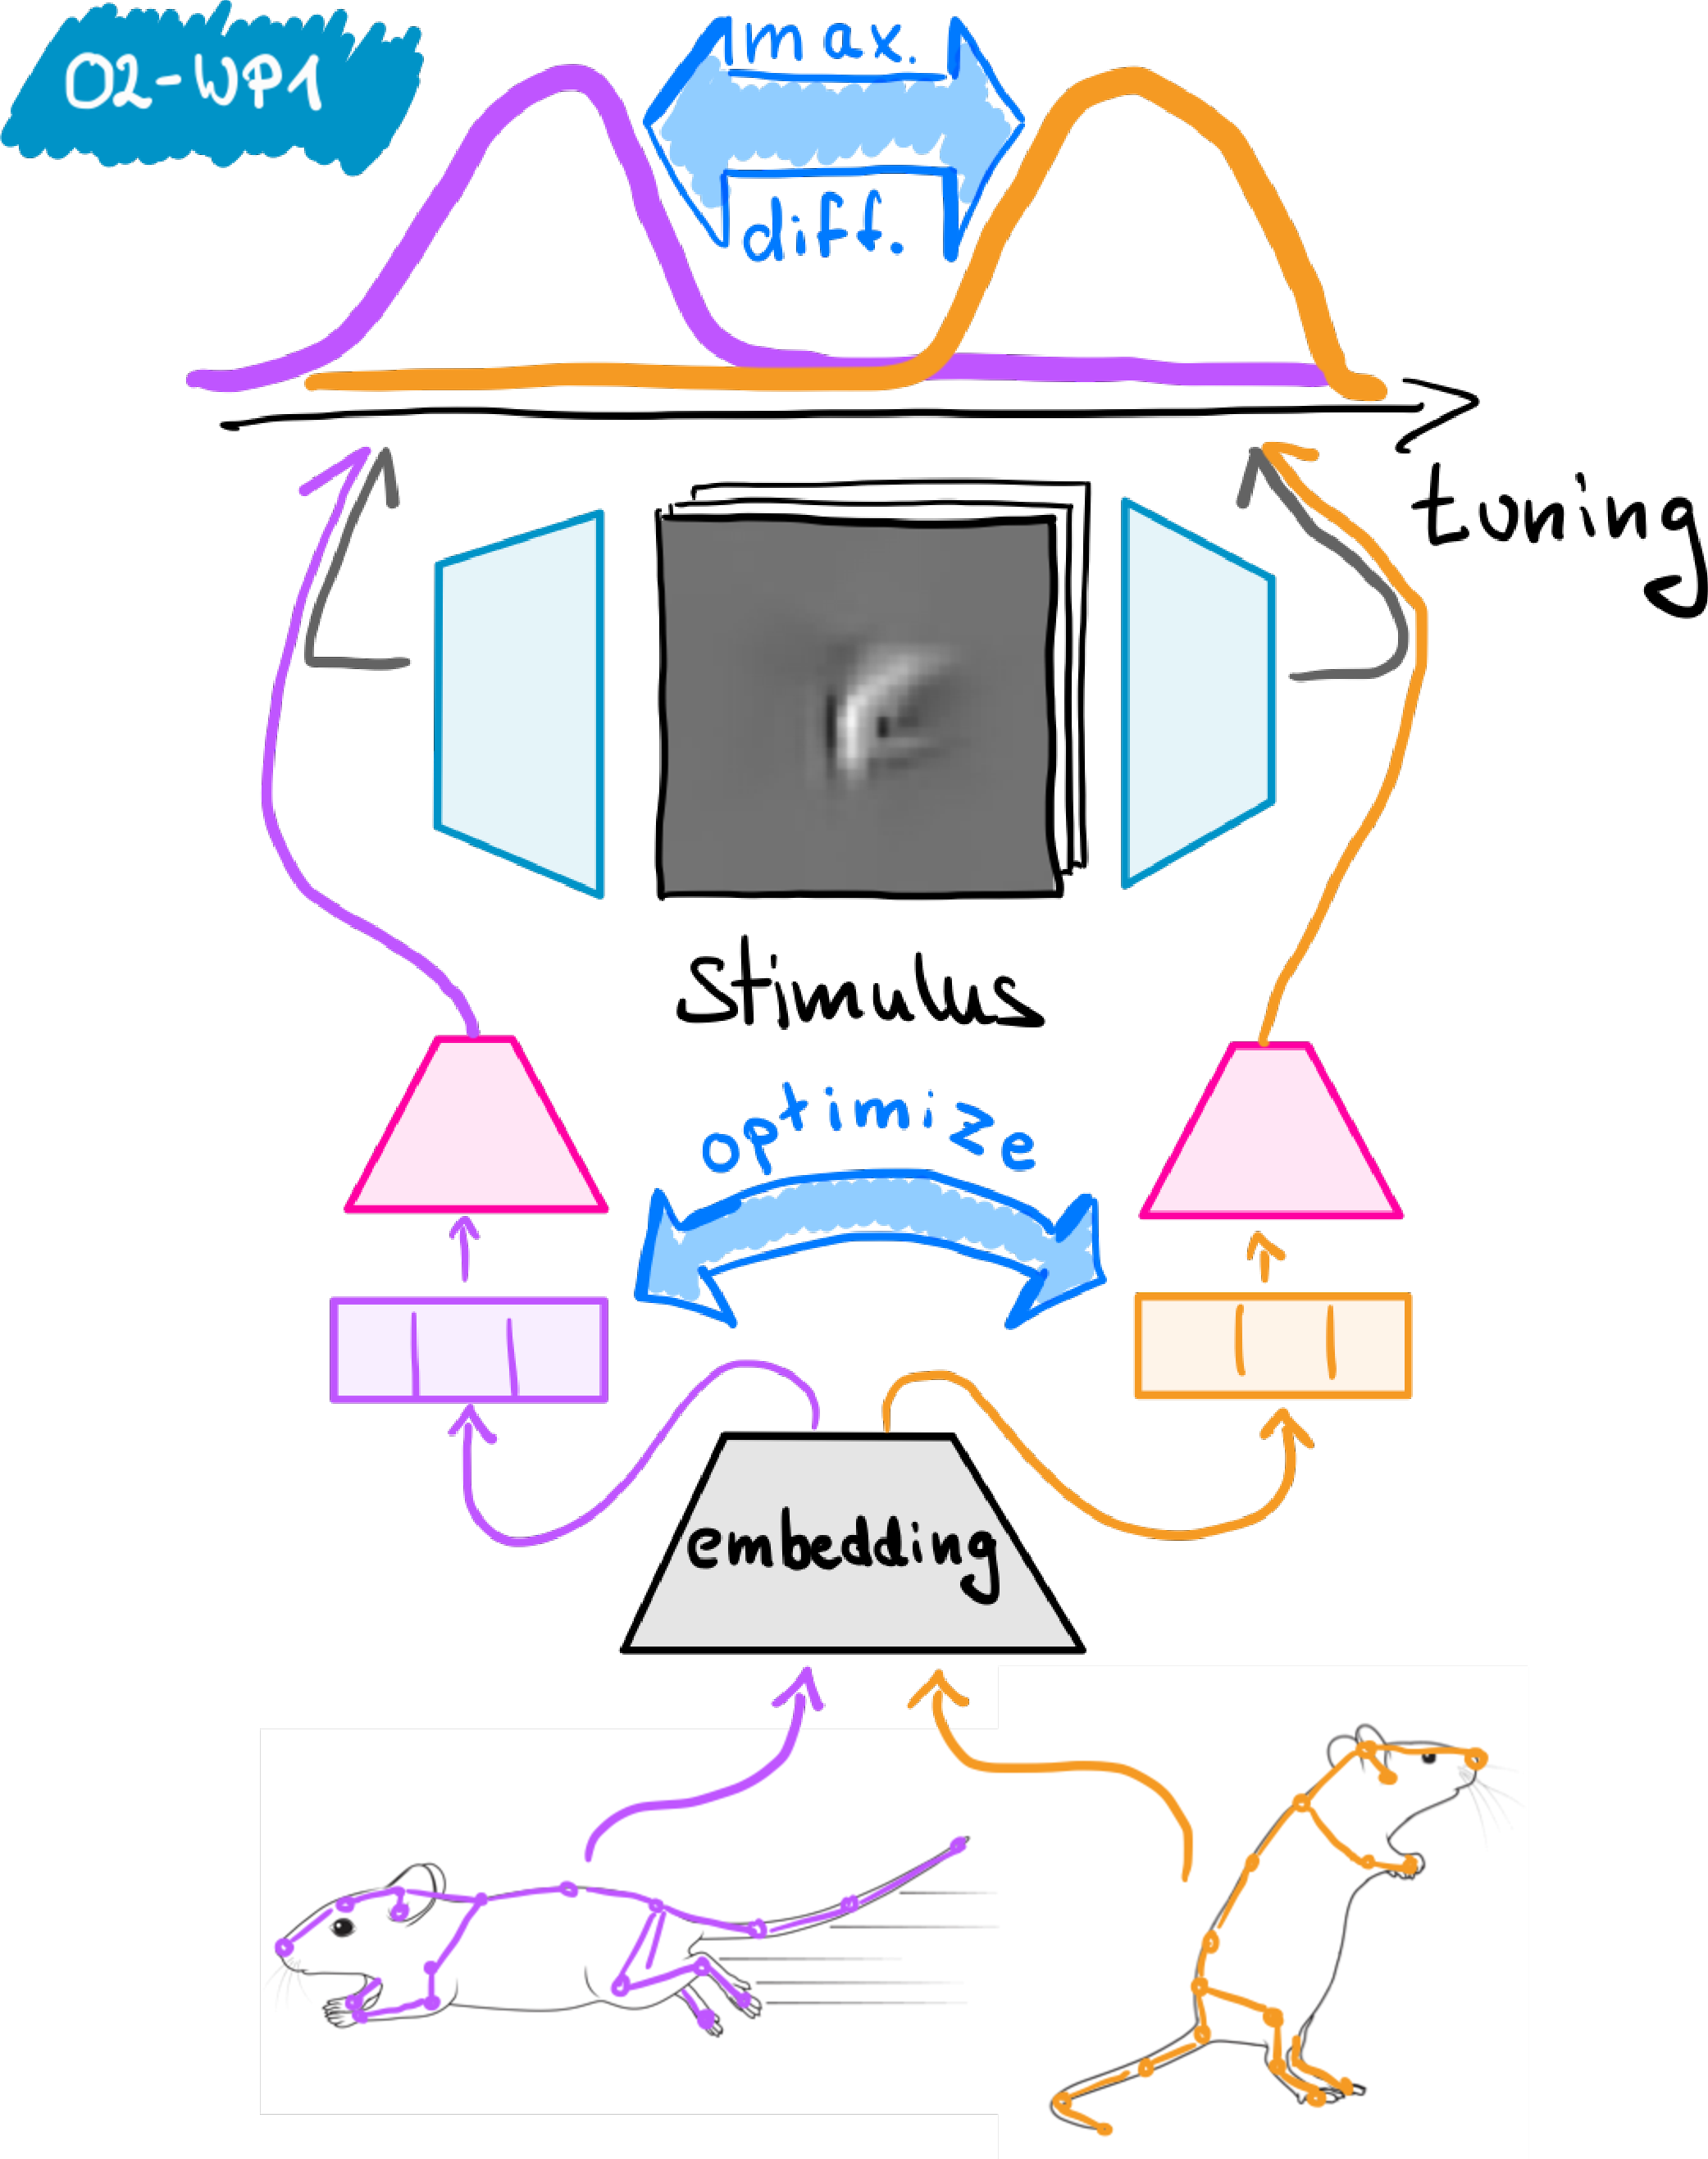
\includegraphics[width=\linewidth]{figures/o2wp1.pdf}
\caption{Find correspondence between behavior and tuning.\label{fig:o2wp1}}
\end{wrapfigure}
%
Because the tracked keypoints in 3D are correlated in space and time, they can be more compactly described in behavioral motifs. 
To extract these motifs form the data, we will first fit a latent state probabilistic model to the trajectories of the 3D graphs to describe them in terms of a low dimensional continuous latent state and a clustering of those embedding into discrete motifs~\parencite[similar to][]{Wiltschko2015-ey, Wiltschko2020-zd}.
Since this model can also generate 3D graphs, we will connect it the model of~\objwp{1}{1} to make it a function of a stimulus and the latent behavioral embedding: \texttt{neural responses = model(video stimulus, 3D postures(embedding))}.
Note that the video stimulus would usually be a function of the 3D postures and eye movements, which determine where the animal looks. 
However, our functional twin models allows us to decouple the stimulus from the behavior and use it to find pairs of stimuli and embedding vectors (and their corresponding 3D posture trajectory) to map out tuning changes of single neurons with respect to motor behavior. 
To this end, we will first describe the tuning manifold of each neuron, by extending a contrastive learning algorithm we developed~\parencite{Baroni2022-fi}, and then find directions in the behavior embedding space that maximally modulate the response of a given neuron to this stimulus manifold, i.e. change its tuning (Fig.~\ref{fig:o2wp1}).
This can be done using optimization on the embedding space. 
To visualize the changes in tuning, we will compute maximally exciting video~\parencite{Walker2019-yw} for each extreme in the behavior embedding space. 
In addition to motor behavior, task context could explain tuning changes. 
To account for this possible confounder, we will add task variables (trial active or not, what object ID was shown, etc.) as additional variables to the model in the same way we added behavior, and then condition on the task context first to see whether motor behavior can explain tuning changes beyond task context. 
If task context has an influence, we will also analyze how it changes tuning in the same way we analyzed the motor behavior. 
Together with our experimental partners, we will experimentally verify the predicted change in tuning by designing stimuli that can will yield differential responses under the different behavioral states irrespective of gaze. 

\subsubsection{Workpackage 2.2: Reconstruct scene features under tuning extremes. \hfill \objwp{2}{2}}
\labelobjwp{2}{2}
% One of the objectives of stochastic optimal control is to reduce the uncertainty about the state determined (among others senses) by the visual system. 
% Since not every aspect of the environment is equally important for every behavior, we hypothesize that tuning changes corresponding do different behavioral motifs found in~\objwp{2}{1} also affect the certainty about different stimulus dimensions. 
\begin{wrapfigure}[9]{r}{.6\textwidth}
\includegraphics[height=.24\linewidth]{figures/random_scene.png}

\includegraphics[height=.24\linewidth]{figures/random_scene_segmentation.png}

\includegraphics[height=.24\linewidth]{figures/random_scene_depth.png}
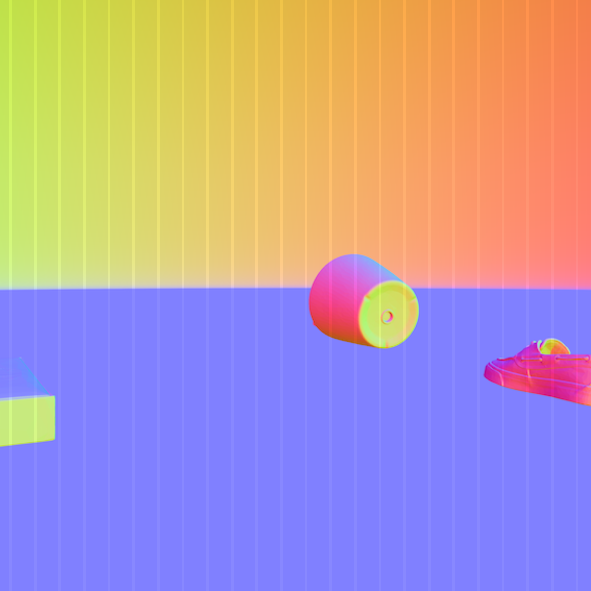
\includegraphics[height=.24\linewidth]{figures/random_scene_surface_normals.png}
\caption{Rendered scene with scene properties: segmentation, depth, and (one angle of) surface normals.\label{fig:o2wp2}}
\end{wrapfigure}
Modulation or change in tuning of visual neurons usually goes hand in hand with increased signal quality and better behavioral performance \parencite{Spitzer1988-kq, Bennett2013-rk, Dadarlat2017-jw, De_Gee2022-ir}.
I thus expect any change in tuning found in~\objwp{2}{1} to also increase signal quality specific dimensions.
Since the goal of the visual system is to infer information about the \textit{world}, not the \textit{image}, we will analyze what these dimensions are in terms of scene features. 

To investigate this, we will reconstruct scene features, such as object boundaries, depth, curvature, slant, texture, and optical flow (Fig.~\ref{fig:o2wp2}), that are available to us in the digitized scene and the rendered stimuli from object recognition task, under the different tuning extremes identified in~\objwp{2}{1}.
To that end, we will train another convolutional or recurrent feature map (\texttt{FM}, Fig~.\ref{fig:model}) of the network from~\objwp{1}{1} to reproduce the features of the original core by minimizing the difference between 
% \begin{center}
    \texttt{FM\_old(rendered video)} and \texttt{FM\_new(scene properties)}
% \end{center}
with respect to the parameters (network weights) of \texttt{FM\_new}. 
Note, that this does not require neural responses to rendered stimuli, only pairs of rendered videos and latent dimensions, which are cheap to generate. 
We have previously demonstrated that matching the outputs of a core can reproduce the essential features for neural prediction~\parencite{Safarani2021-yy}.
This yields a new model \texttt{neural responses = model(\textbf{scene properties}, 3D postures(embedding))}.
We can then decode the world properties from neural responses by optimizing them to match the real neuronal response using the model and different behavioral motifs.
We have previously demonstrated with models for static natural images and verification experiments~\parencite{Cobos2022-rr}, that this approach best captures the perceptual relevant dimensions for mouse visual cortex. 
We will then analyze the accuracy and variability with which different world properties are decoded under different behavioral states. 

\subsubsection{Expected outcome} 
I expect to find changes in tuning that correspond to particular behavioral motifs, and possibly task context.
Irrespective of what caused the change in tuning, I expect that the behavioral context determines which scene features are better decodable from the model, \ie decrease uncertainty in specific dimensions.
I expect these dimensions to be meaningful with respect to the behavioral context. 
For example, object boundaries or non-self-induced optic flow could be enhanced during running. 
% Other possible changes could be that neurons become more invariant to optic flow generated by the own movement of the animal \hl{how would we exactly find that?}, 

\subsubsection{Risk management} 
The goal of this objective is to find new correspondences between change in tuning of neurons in visual cortex and particular behavioral contexts in freely moving animals in a data-driven way.
It is conceivable that we will not find any new mechanisms.
However, given that \textcite{Stringer2019-lt} showed that by just including more features from the face of the mouse explains more variance in spontaneous activity of head-fixed mice than simple arousal variables like running, pupil, or whisking, it is highly unlikely that detailed motor behavior will not explain any of the latent changes in neuronal activity. 
In that case, this objective will still yield valuable output because it still allows us to describe \textit{when} modulation of neuronal activity occurs in freely behaving animals under natural stimulation, and how this relates to latent scene variables. 




%%%%%%%%%%%%%%%%%%%%%%%%%%%%%%%%%%%%%%%%%%%%%%%%%%%%%%%%%%%%%%%%%%%%%%%%%%%%%%
\subsection{\colorbox{obj3}{\color{white} O3} Objective 3: \othreetitle .}
\labelobj{3}

\textbf{Goals:} Build a computational framework based on reinforcement learning to predict how an animal would change its behavior as a result of (experimental) manipulations of neurons in visual cortex. Use this framework to predict how behavior of an animal would be different if behavior-associated changes in tuning were disabled. 

\textbf{Overview and rationale:} 
Previous studies reported that modulation of sensory responses resulted in better behavioral performance \parencite{Spitzer1988-kq, Bennett2013-rk, Dadarlat2017-jw, De_Gee2022-ir}, suggesting that they are necessary for successful behavior. 
% I thus hypothesize that tuning changes in general bias visual processing towards task- or behavioral relevant signals.
\obj{2} identified how changes in tuning \textit{correlate} with behavior, but did not demonstrate whether they are \textit{necessary} for the animal to perform certain tasks.
% However, to determine whether these changes are relevant for downstream mechanisms to determine behavior, we need to establish \textit{necessity}. 
The goal of this objective is to build a computational framework to predict how motor behavior and task performance of an animal would change if temporary changes in tuning, supposed to adapt the visual system to behavioral context, were disabled.  
% This a challenging causal and counterfactual question that involves the \textit{prediction} of full behavioral trials of an animal
The difficulty for making such a prediction results from the redundancy of the visual stimulus and the visual system: 
Even when a particular neural mechanism is suppressed or altered, there might be other ways for the animal to still achieve the behavioral goal. 
To model the effect of changes in visual representations on behavior in open field behavior, we need to account for the possibility that the animal chooses a different strategy to still solve the same task. 
This means, we need to allow our model to change its behavior to solve the task. 
To that end, I propose use the functional twin of in combination with reinforcement learning.
The reinforcement learning agent will have the previously learned visual system of a mouse (with and without manipulations) to access the state of the environment.
The learned behavioral policy of the agent will make predictions about the behavior of the animal. 
When the manipulation is turned on, the agent can either use the previously learned policy or adapt the policy to compensate for the changes in the visual system.
Both will make a prediction about the change in behavior of the animal. 
% To account for this, I propose to build a reinforcement learning agent based on the functional twin and let it learn to solve an open field recognition task in the digitized environment. 
% The behavioral policy of this agent will make a prediction about the animal's behavioral strategy and performance.
% Simulating experimental interventions on the visual system of the agent and letting it solve the task again, will then allow me to make predictions how the behavior changes under experimental interventions. 
% As a consequence, the behavioral changes might be subtle and thus hard to predict or interpret.

Since this approach is completely novel, we will build it in several steps. 
We will first capture the effect of optogenetic manipulations one the neuronal representations in the model using large scale recordings from head-fixed animals. 
We will then model the effect of these manipulations on the decisions of the mouse in a object recognition task during head-fixed and open field behavior. 
Since we will have the corresponding experimental data this will be a strong test whether our model can indeed capture the effect of causal manipulations on behavior.
Once that is established, we will use this framework to model how the open field behavior will be affected if we disable behavior-associated changes in tuning.

\subsubsection{Workpackage 3.1: Causal manipulations in head-fixed animals\hfill\objwp{3}{1}}
\labelobjwp{3}{1}
We will model the effect of optogenetic inhibition of different areas onto decisions of mice in two alternative forced choice object recognition tasks. 
The data consists of large-scale 2-photon recordings from multiple visual areas in different head-fixed mice performing the object recognition task under normal conditions and when particular areas are optogenetically suppressed.
We will first model whether we can predict the animals decisions under normal conditions. 
To that end, we will train a model to predict the correct outcome for each trial either from the modeled neurons or directly from the feature representation of the functional twin without using the  latent state in the model.
We will then freeze the task decoder, enable the latent state in the visual model and infer its actual state from the neuronal recordings. 
Then we will compare the decisions of the model with the decisions of the animal. 
We expect that adding the latent state will increase the prediction accuracy of the animal's choices. 

In the next step, we will extend the model to account for the effect of optogenetic manipulations. 
To that end, we will include an additional input to the model that indicates whether the manipulation was \textit{on} or \textit{off}. 
We will then only adapt the feature representations of the model (see Fig.~\ref{fig:model}) to account for the changes in neuronal activity to visual stimuli without a task under both conditions.
This will also reflect any changes on neuronal representations on other areas that might be mediated through feedback and do not require the model to be anatomically faithful. 
% Since the optogenetic inhibition will be local, we will add positional encoding to the additional input so the core can change spatially localized. 
Subsequently, we use this model to predict the animals decisions like above, with the additional ability to simulate optogenetic manipulations.
% We will train it with the core where the manipulations are off, and then predict the decisions of the animal when the manipulations are on.
We expect that our model faithfully generalizes and correctly predicts the decisions of the animal. 

\subsubsection{Workpackage 3.2: Predicting effect of optogenetic manipulations in an open field task\hfill\objwp{3}{2}}
\labelobjwp{3}{2}

Predicting the effect of circuit manipulations on task performance and decisions of the animal becomes more challenging in the open field task because we need to account for the entire behavioral trace leading up to the decision. 

\textbf{Modeling decisions:} 
We will put the visual model from \objwp{3}{1} with and without circuit manipulations onto the posture graph from tracked behavior of animals performing the task (as in \obj{1}) and predict miniscope neuronal activity when the optogenetic manipulation is on or off. 
Then we will train an additional decision network to decode the right task outcome like in \objwp{3}{1} and test whether it can predict decisions of the animal depending on the latent state inferred from behavior and neuronal recordings, and the changes in decisions under optogenetic manipulation. 

\textbf{Modeling behavior:} 
Before, we predicted the effect of optogenetic manipulations on the \textit{decisions} of the animal for \textit{actually observed behavior} in the open field task. 
As a next step, we will build a model to predict the change in \textit{behavior} using reinforcement learning.
% However, because the visual representation has changed, the animal might use compensatory strategies which will cause behavior itself to change. 
% In this work package, we want to predict that change in behavior using reinforcement and imitation learning. 
To that end, we will put the model for the visual system on top of a virtual agent and learn how to solve the task with behavior, \ie\ predict the actions of the animal to solve the task (maximize the task reward). 
This will predict \textbf{motor behavior, decisions and task performance} of the animal. 
This step is crucial for \objwp{3}{3} where we want to predict the changes in performance and behavior when turning off behavior-associated tuning changes, since we will not have actually observed behavioral trajectories of the animal under that intervention. 

To predict behavior and performance of an animal in the open field object recognition task, we will use reinforcement learning with phasic policy gradient~\parencite[PPG,][]{Cobbe2021-op}. 
% or imitation learning~\parencite{Chen2021-ap} using the functional twin from \obj{1} in the digitized environment. 
Phasic policy gradient (PPG) is a state-of-the art method for learning behavior with a continuous actions space. 
It has been utilized in the recent work \cite{Baker2022-ph}, which showed that first pre-training a reinforcement learning model using behavioral cloning provides a strong prior over the actions decreasing the exploration space to a more meaningful domain. 
As a result, the following fine-tuning using PPG is more efficient and gives rise to more complex behaviors than were previously possible with reinforcement learning only.
We will use the functional twin's visual model response to the rendered frames from the mouse's point of view as state observations for the reinforcement learning model (either the feature map + latent state or the neurons directly), followed by a classifier for modeling the policy over binned actions.
Similarly to \cite{Baker2022-ph}, we will then train a foundation model for predicting actions using behavioral cloning i.e. maximizing the likelihood of the actions performed by the mouse given the rendered images.
Using the real runs for pre-training the behavioral model decreases the initial exploration complexity and provides a meaningful base policy.
We will then fine-tune the foundation model using simulated experiments and reinforcement learning. 
To that end we will simulate the behavior of the mouse in the virtual environment and we will update the policy using phasic policy gradient \parencite{Cobbe2021-op} to maximize the reward obtained in the environment.

We will then analyze two cases: In the first, we train the agent on the unmanipulated visual model and turn on the manipulation during test time. 
This will model the situation where the animal has not yet adapted its behavior to the manipulation of the circuit. 
In the other case, we will learn another policy with the manipulated visual model so the agent can learn to adapt its behavior to the changed visual system. 
This will model the situation where the animal has potentially developed a different strategy to solve the task. 
We will quantify how well our approach predicts the behavior by training a classifier that has to distinguish between real trials of the animal and trials generated by our agent. 
Given the trained model, we can then analyze where the behavior maximally differ by comparing the decisions of the policy classifier under the manipulated and un-manipulated conditions. 

\subsubsection{Workpackage 3.3: Predicting behavioral relevance of tuning changes\hfill\objwp{3}{3}}
\labelobjwp{3}{3}

After we have validated the framework in \objwp{3}{2}, we will use the model to predict behavioral changes and changes in performance when manipulating behavior-associated changes in the model. 
To achieve this in the model, we can simply pretent to the latent state that the agent performed a different behavior than it actually did, thus controlling the associated change in tuning. 
The agent will still take a particular action to achieve the goal, but the feedback to the visual system will get a different behavior, particularly the one we identified in \objwp{2}{2}.
Then we will repeat the same procedure as in \objwp{3}{2} to predict behavioral and performance changes of the animal under this manipulation. 
The quantification will be the same as in \objwp{3}{2}.
To experimentally test our predictions together with our experimental partners, we will optimize a stimulus manipulation (\eg~a degrade in quality in the scene predicted by \objwp{2}{2}) that simulates tuning off the change in tuning. 
Then we will display this stimulus in the respective behavioral episodes (\eg~blur the edges when the animal runs) and test whether we can get a similar behavior as predicted by our agent.

\subsubsection{Expected outcome} 
In \objwp{3}{1} and \objwp{3}{2} I expect that adding the latent state in the model can better explain the decisions of the animal, and that modeling the changes of the optogenetic manipulations to the visual system can account for changes in decisions and motor behavior. 
In \objwp{3}{3}, I expect that our framework predicts a loss in performance when behavior associated tuning changes are turned off but the original behavioral policy is kept, because -- according to my hypothesis -- the agent (animal) cannot benefit from a decrease of uncertainty in behaviorally relevant scene properties anymore. 
In particular, I expect that en- and disabling tuning changes mostly affects behavior/performance when their associated behavioral motifs are actively used in the task, or when the have been identified to occur in the context of the task (in \obj{2}).
When we learn a new policy using the visual system without tuning changes, I expect the performance to partly recover, but I expect the agent to come up with motor behavior, that can compensate the loss in certainty. 
For instance, the agent could take longer to decide to trade off the loss in certainty with longer observation times. 


\subsubsection{Risk management} 
The approach of combining a large scale model of the visual system with behavioral predictions of new behavior via reinforcement learning is novel and thus has the potential to fail. 
To de-risk the possibility of failure, I intentionally designed \obj{3} in stages of increasing complexity and difficulty. 
Existing work provides evidence that the intermediate likely be successful.  
For instance, \textcite{Kalweit2022-ev} combined inverse reinforcement learning with neuronal data and showed that they can predict actual behavior of a rat better, even under experimental interventions. 
All of these stages will yield interesting insights on their own and help to diagnose why a particular next stage failed and eventually lead to the fix of that problem. If the agent should fail to emulate behavior of individual mice, we will ``personalize'' the agent to these mice by low-dimensional adjustments in the reward structure~\parencite{Kwon2020-qb}.

\subsection{Dissemination}
Results and algorithms from this project will be published on peer reviewed conference proceedings or journals. 
Conference proceedings will be open access.
For journals, we will upload a preprint to arXiv or bioRxiv prior to submission, as we have done with the majority of our research in the last years. 
In addition, we will organize workshops on the topic of functional and digital twins at conferences such as CoSyNe, Fens, Society for Neuroscience Meeting, or Bernstein Conference for Computational Neuroscience.
In addition, it is standard practice in my lab to release the code, software libraries and trained models along with the publication on GitHub.
Whenever it makes sense, we also provide a Docker container with a trained model to run our models in an reproducible environment without the need to install extra dependencies. 

\subsection{Team and Timeline}
The project work will be carried out by a postdoc (\circled[postdoc1][postdoc1][postdoc1]{a}), and two PhD students (\circled[phd1][phd1][phd1]{a} and \circled[phd2][phd2][phd2]{a}). 
PhD student \circled[phd1][phd1][white]{1} will develop the functional twin for \obj{1} and work with the postdoc to adapt it to the optogenetic manipulations in \objwp{3}{2}.
PhD student \circled[phd2][phd2][white]{2} will find and interpret the behavior associated changes in tuning \obj{2}, and work with the postdoct to assess the causal effect of disabling these tuning changes on behavior in \objwp{3}{3}.
The postdoc \circled[postdoc1][postdoc1][postdoc1]{a} will focus on the aspects involving reinforcement learning and manipulations (\objwp{1}{2} and \obj{3}). 
Together with me, (s)he will also supervise both PhD students.
I will supervise the entire project.

\begin{ganttchart}[
    y unit chart=.4cm,
    x unit=3.2mm,
    y unit title=.5cm,
    canvas/.append style={fill=none, draw=black!5, line width=.75pt},
    hgrid style/.style={draw=black!20, line width=.75pt,},
    vgrid={*{3}{dotted},*{1}{dashed},
           *{3}{dotted},*{1}{dashed},
           *{3}{dotted},*{1}{dashed},
           *{3}{dotted},*{1}{dashed},
           *{3}{dotted},*{1}{draw=black!100, line width=1pt}
            },
    % today=,
    today rule/.style={
      draw=black!64,
      dash pattern=on 3.5pt off 4.5pt,
      line width=1.5pt
    },
    today label font=\footnotesize\bfseries,
    title/.style={draw=none, fill=none},
    title label font=\bfseries\footnotesize,
    % title label node/.append style={below=7pt},
    include title in canvas=false,
    bar label font=\mdseries\footnotesize\color{black!70},
    bar label node/.append style={left=.2cm},
    % bar/.append style={draw=none, fill=black!63},
    bar/.append style={draw=none},
    bar progress label font=\mdseries\footnotesize\color{black!70},
    milestone label font=\mdseries\footnotesize\color{black!70},
    milestone label node/.append style={left=.2cm},
    group/.append style={fill=black},
    group left shift=0,
    group right shift=0,
    group height=.2,
    group peaks tip position=0,
    group label node/.append style={left=.2cm},
    group label font=\bfseries\small,
  ]{1}{20}
  \gantttitle[
    title label node/.append style={left=7pt}
  ]{Years:}{0}
  \gantttitle{1}{4} 
  \gantttitle{2}{4}
  \gantttitle{3}{4}
  \gantttitle{4}{4}
  \gantttitle{5}{4}\\
  \ganttgroup{Objective 1: A data-driven embodied digital twin}{1}{16} \\
  \ganttbar[bar/.append style={fill=postdoc1}]{Supervision of PhD-1}{1}{16}\\
  \ganttbar[bar/.append style={fill=phd1}]{\objwp{1}{1} A video-driven latent state model of the visual system}{1}{6}\\
  \ganttbar[bar/.append style={fill=postdoc1}]{\objwp{1}{2} Digitizing the environment and tracking behavior}{1}{6}\\
  \ganttbar[bar/.append style={fill=phd1}]{\objwp{1}{3} Functional twin with behavior}{5}{10}\\
  \ganttnewline[solid, gray]
  \ganttgroup{Objective 2: Tuning changes}{5}{20} \\
  \ganttbar[bar/.append style={fill=postdoc1}]{Supervision of PhD-2}{5}{20}\\
  \ganttbar[bar/.append style={fill=phd2}]{\objwp{2}{1} Find behavior-associated change in visual tuning}{5}{12}\\
  \ganttbar[bar/.append style={fill=phd2}]{\objwp{2}{2} Reconstruct scene features under tuning extremes}{12}{20}\\
  \ganttnewline[solid, gray]
  \ganttgroup{Objective 3: Causal model for behavioral change}{5}{20} \\
  \ganttbar[bar/.append style={fill=postdoc1}]{\objwp{3}{1} RL with embodied twin}{5}{14}\\
  \ganttbar[bar/.append style={fill=phd1}, bar top shift=0.5]{\objwp{3}{2} Effect of causal manipulations}{11}{16}
  \ganttbar[bar/.append style={fill=postdoc1}]{}{13}{18}\\
  \ganttbar[bar/.append style={fill=phd2}, bar top shift=0.5]{\objwp{3}{3} Effect of tuning change}{13}{16}
  \ganttbar[bar/.append style={fill=postdoc1}]{}{15}{20}\\
\end{ganttchart}


%%%%%%%%%%%%% BIBLIOGRAPHY %%%%%%%%%%%%%%%%%%%
\begin{small}
\printbibliography
\end{small}

% \renewcommand\bibsection{\subsection{\refname}}
% \begin{small}
% 	\bibliographystyle{aa}
% 	\bibliography{bibliography}
% \end{small}

%%%%%%%%%%%%% CURRICULUM VITAE %%%%%%%%%%%%%%%%%%%

\end{document}